\documentclass[crop=false]{standalone}
%\documentclass{standalone}
\usepackage{tikz} % To generate the plot from csv
\usepackage{pgfplots}
\usepackage{graphicx}
\usepackage{booktabs}
\usepackage{subfig}
\usepackage{float}
\usepackage[section]{placeins} % getting figures below sections
\usepackage{blindtext}
\usepackage{siunitx}
\usepgfplotslibrary{units} % Allows to enter the units nicely
\usetikzlibrary{external} %https://tex.stackexchange.com/questions/1460/script-to-automate-externalizing-tikz-graphics
\tikzexternalize[prefix=savedfigures/]

\pgfplotsset{compat=newest} % Allows to place the legend below plot
\usepackage{pgfplotstable}
\usepgfplotslibrary{statistics}

% #################### Function definition for box plots read table ##################\
\makeatletter
\pgfplotsset{
	boxplot prepared from table/.code={
		\def\tikz@plot@handler{\pgfplotsplothandlerboxplotprepared}%
		\pgfplotsset{
			/pgfplots/boxplot prepared from table/.cd,
			#1,
		}
	},
	/pgfplots/boxplot prepared from table/.cd,
	table/.code={\pgfplotstablecopy{#1}\to\boxplot@datatable},
	row/.initial=0,
	make style readable from table/.style={
		#1/.code={
			\pgfplotstablegetelem{\pgfkeysvalueof{/pgfplots/boxplot prepared from table/row}}{##1}\of\boxplot@datatable
			\pgfplotsset{boxplot/#1/.expand once={\pgfplotsretval}}
		}
	},
	make style readable from table=lower whisker,
	make style readable from table=upper whisker,
	make style readable from table=lower quartile,
	make style readable from table=upper quartile,
	make style readable from table=median,
	make style readable from table=average,
	make style readable from table=lower notch,
	make style readable from table=upper notch
}
\makeatother
\begin{document}

\section{23 2 Mumford0 SA Mutations AMALGAM 20210815 221256}
Removed 0 and 7

% ######################## UTRP SA Mutation operators applied ######################## 
\begin{figure} 
\centering 
\tikzsetnextfilename{UTRP_DBMOSA_BP_mutation_funcs_Counts_normal_phd} 
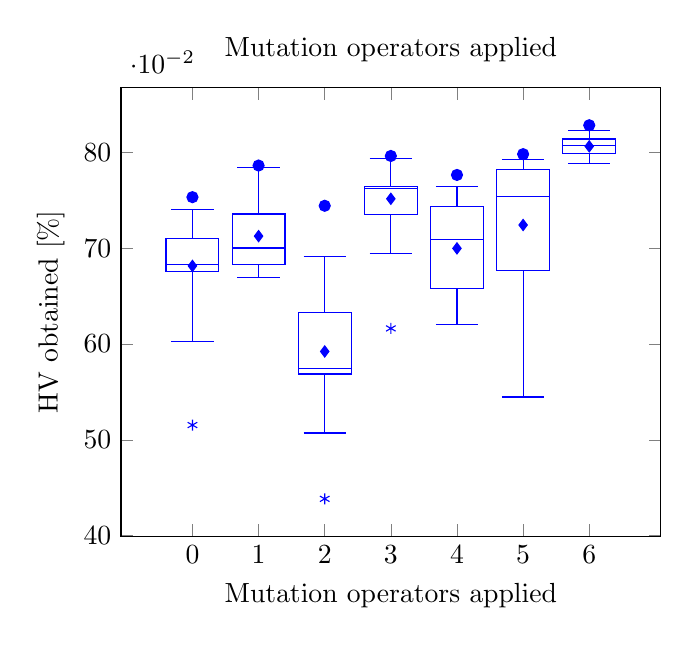
\begin{tikzpicture} 
\begin{axis}[ 
title={Mutation operators applied}, 
boxplot/draw direction=y, 
xtick={1,2,3,4,5,6,7}, 
xticklabels={0,1,2,3,4,5,6}, 
x tick label style={rotate=0, align=center}, 
xlabel={Mutation operators applied}, 
%y tick label style={/pgf/number format/.cd,fixed,precision=3, zerofill}, 
scaled y ticks={base 10:2},
ylabel={HV obtained [\%]}, 
] 

% ############## Mutations_Counts_normal=1 ################## 
\addplot[boxplot, mark=asterisk, 
boxplot prepared={ 
lower whisker=0.60252, 
upper whisker=0.73995, 
lower quartile=0.67515, 
upper quartile=0.71025, 
median=0.68305, 
average=0.68138}, 
color = blue, solid, area legend] 
coordinates {
(1,0.51539)}; 
\addplot[only marks,mark=*,color = blue]coordinates{(1,0.75313)}; 

% ############## Mutations_Counts_normal=2 ################## 
\addplot[boxplot, mark=asterisk, 
boxplot prepared={ 
lower whisker=0.66921, 
upper whisker=0.78377, 
lower quartile=0.6831, 
upper quartile=0.73551, 
median=0.70013, 
average=0.71247}, 
color = blue, solid, area legend] 
coordinates {}; 
\addplot[only marks,mark=*,color = blue]coordinates{(2,0.78613)}; 

% ############## Mutations_Counts_normal=3 ################## 
\addplot[boxplot, mark=asterisk, 
boxplot prepared={ 
lower whisker=0.50711, 
upper whisker=0.69107, 
lower quartile=0.5686, 
upper quartile=0.63234, 
median=0.57397, 
average=0.59218}, 
color = blue, solid, area legend] 
coordinates {
(3,0.4384)}; 
\addplot[only marks,mark=*,color = blue]coordinates{(3,0.74415)}; 

% ############## Mutations_Counts_normal=4 ################## 
\addplot[boxplot, mark=asterisk, 
boxplot prepared={ 
lower whisker=0.69392, 
upper whisker=0.79316, 
lower quartile=0.73491, 
upper quartile=0.76383, 
median=0.76194, 
average=0.75145}, 
color = blue, solid, area legend] 
coordinates {
(4,0.6162)}; 
\addplot[only marks,mark=*,color = blue]coordinates{(4,0.79611)}; 

% ############## Mutations_Counts_normal=5 ################## 
\addplot[boxplot, mark=asterisk, 
boxplot prepared={ 
lower whisker=0.62038, 
upper whisker=0.7645, 
lower quartile=0.65756, 
upper quartile=0.74382, 
median=0.70934, 
average=0.6997}, 
color = blue, solid, area legend] 
coordinates {}; 
\addplot[only marks,mark=*,color = blue]coordinates{(5,0.77631)}; 

% ############## Mutations_Counts_normal=6 ################## 
\addplot[boxplot, mark=asterisk, 
boxplot prepared={ 
lower whisker=0.54466, 
upper whisker=0.79277, 
lower quartile=0.67635, 
upper quartile=0.7817, 
median=0.7536, 
average=0.72407}, 
color = blue, solid, area legend] 
coordinates {}; 
\addplot[only marks,mark=*,color = blue]coordinates{(6,0.79802)}; 

% ############## Mutations_Counts_normal=8 ################## 
\addplot[boxplot, mark=asterisk, 
boxplot prepared={ 
lower whisker=0.78859, 
upper whisker=0.82303, 
lower quartile=0.79904, 
upper quartile=0.8138, 
median=0.80677, 
average=0.80617}, 
color = blue, solid, area legend] 
coordinates {}; 
\addplot[only marks,mark=*,color = blue]coordinates{(7,0.82817)}; 

\end{axis}
\end{tikzpicture}
\end{figure} 
\begin{table}
\centering
\caption{Legend for the boxplot.}
\begin{tabular}{ll}
\toprule
 Index &                                               Name \\
\midrule
     0 &               [MSC\_add\_terminal, MSC\_del\_terminal] \\
     1 &                        [Add\_vertex, Delete\_vertex] \\
     2 &       [Trim\_one\_terminal\_cb, Grow\_one\_terminal\_cb] \\
     3 &       [Insert\_inside\_vertex, Delete\_inside\_vertex] \\
     4 & [Add\_vertex, Delete\_vertex, Insert\_inside\_verte... \\
     5 &        [Add\_vertex, Delete\_vertex, Intertwine\_two] \\
     6 & [Add\_vertex, Delete\_vertex, Insert\_inside\_verte... \\
     7 & [MSC\_add\_terminal, MSC\_del\_terminal, Insert\_ins... \\
     8 & [Add\_vertex, Delete\_vertex, Insert\_inside\_verte... \\
\bottomrule
\end{tabular}
\end{table}

\end{document}
